

\begin{abstract}
    abstract
\end{abstract}

\minitoc


\section{Introduction}

% The SPRA contains several tools and things

The Seismic Probabilistic Risk Assessment (SPRA) defines a framework and a methodology for the study of seismic structural reliability. %This framework is parrt of the probabilistic 
% As for the Pr
It has been introduced since 1969 \citep{cornell_engineering_1968}
to incorporate the seismic risk evaluation in the probabilistic risk assessment studies.
% and further developed in the
The SPRA has been mostly developed and carried out in the 1980s on nuclear facilities (see e.g. \cite{kennedy_probabilistic_1980,kennedy_seismic_1984}). 
It includes: the determination of the seismic hazard, the analysis of the seismic fragility of structural components, the evaluation of the risks combination and their consequences in the system, as described in the report of the Electric Power Research Institute \citep{epri_seismic_2013}, which provides guidelines for its implementation. %among other ingredients.
%The guidelines for its implementation are thoroughly described in the 
It is since widely used in the nuclear industry (e.g. \cite{ellingwood_validation_1990,park_survey_1998,kennedy_risk_1999}) and its consideration is established among the safety standards adopted by the International Atomic Energy Agency \citep{iaea_probabilistic_2020}.

% Estimating th

Within the SPRA, seismic fragility curves represent a key asset that play a prominent role in the analysis of structural components' fragility step (see  \cite{epri_advanced_2011}).
They express in probabilistic terms the fragility of structures under seismic excitation. We can mention that they are also a tool of interest of performance-based earthquake engineering (PBEE; \cite{ghobarah_performance-based_2001,noh_development_2014}), 
which aims at relating performance objectives to level of damage to the structure.
In any case, they are defined as a function of the seismic hazard, which ---driven by the magnitude (M), the source-site distance (R), and other earthquake parameters--- is reduced to a scalar value derived from the seismic signal: the intensity measure (IM), under the so-called ``sufficiency assumption'' \citep{cornell_hazard_2004,luco_structure-specific_2007}.
In practice, a fragility curve, denoted $P_f$, therefore express the probability of failure of a mechanical structure as a function of an IM value of interest such as peak ground acceleration (PGA) or pseudo-spectral acceleration (PSA), among others:
    \begin{equation}
        P_f(a) = \PP(\text{``failure''}|\text{IM}=a).
    \end{equation}
Within the SPRA framework, the fragility curve expression is expected to be combined with the seismic hazard frequency to compute the damage frequency of the component $C_f$:
    \begin{equation}
        C_f =  \int_0^\infty P_f(a)dH(a).
    \end{equation}
If $H$ is the mean annual  distribution of the IM, $C_f$ represents the annual damage frequency of the component.
It should be noted that the sufficiency assumption was introduced to reduce estimation costs since it assumes that the fragility curve of a given structure is identical regardless of the seismic scenario.
Actually, this assumption embeds some uncertainty in the problem since, as shown in \citeauthor{radu_earthquake-source-based_2018}, \citeyearlink{radu_earthquake-source-based_2018,grigoriu_are_2021}, %\cite{radu_earthquake-source-based_2018,grigoriu_are_2021}, 
different seismic scenarios can lead to identical distributions of some IMs, despite having significantly different frequency contents.
The uncertainty rooted in the fragility curve by this assertion can be classified as an \emph{aleatoric} (irreducible) kind of uncertainty
 (we refer to the \cref{chap:intro-english} for the definition of the uncertainty quantification framework).
% belong to the category of
%The evaluation of the fragility curve defined in eq?? implies the consideration of this
% Focusing the definition of the fragility curve <


In this second part of the manuscript, we focus on the estimation of seismic fragility curves. 
Thus, we do not question the determination of the seismic hazard distribution $H$, nor the derivation of the damage frequency of the component $C_f$.
Nevertheless, estimating the fragility curve itself %for given mechanical equipment 
remains a daunting task. It is commonly done statistically, using different kind of methods depending 
on the source of data available, their characteristics, and their quantity.
This chapter proposes a review of these methods. 
In the next section,
we define the different kind of data involved in the seismic fragility curve estimation in the literature. In particular, we present a stochastic seismic signal generator, and  we present how the failure of mechanical equipment is generally defined.
In section ?? and section ?? different modeling of the fragility curves for its statistical estimation are presented, they are grouped in two categories: non-parametric and parametric.
Explicit examples of case studies are given in section ??, from a theoretical one to an experimental one for which really few data are available.
Given those and the non-exhaustive list of modeling we present from the literature, we question 





% steps of seismic hzarad determination or r
% The derivation 




% it embedds uncertainty suinc...

% that in the step
%As shown in \cite{Radu2018,Grigoriu2021}, different seismic scenarios can however lead to identical distributions of some IMs, although the underlying seismic signals have significantly different frequency contents. As a result, the sufficiency assumption is not met, especially for non-linear, multimodal structures, etc., with current IMs. 
%
%
% Despite this, it is possible to focus on the definition of the resulting fragility curve, without taking the assumption for granted, which is the case in this work.

% and is widely used in in the nuclear industry







% Seismic fragility curves represent a key one. They were introduced in the 1980s for seismic risk assessment studies carried out on nuclear facilities \citep{kennedy_probabilistic_1980,kennedy_seismic_1984,ellingwood_validation_1990,park_survey_1998,kennedy_risk_1999,cornell_hazard_2004}.


% %IN the SPRA, historic, lot of things are defined,
% %among them, the seismic fragility curves. 
% %They represent an essential tool..
% Also used in PBEE, link with insurance?

% IM, sufficientcy assumption. Different, various scenario and methods
% Quantification of uncertainty?


% This chapter suggests a review of the main methods that exist in the literature 




\section{Data: from seismic signals to equipments failures}





In the literature, different source of data are exploited to estimate seismic fragility curves. 
We can cite, for instance:
(i) expert assessments supported by test data (e.g. \cite{kennedy_probabilistic_1980,kennedy_seismic_1984,zentner_fragility_2017}), (ii) experimental data (e.g. \cite{park_survey_1998}), (iii) empirical data from past earthquakes (e.g. \cite{shinozuka_statistical_2000,straub_improved_2008,lallemant_statistical_2015,buratti_empirical_2017,laguerre_empirical_2024}), and (iv) analytical results obtained from various numerical models using artificial or natural seismic excitations (e.g. \cite{ellingwood_earthquake_2001,kim_development_2004,zentner_numerical_2010,koutsourelakis_assessing_2010,mai_seismic_2017,trevlopoulos_parametric_2019,wang_influence_2020,mandal_seismic_2016,wang_seismic_2018,wang_bayesian_2018,zhao_seismic_2020,katayama_bayesian-estimation-based_2021,gauchy_importance_2021,khansefid_fragility_2023,lee_efficient_2023}).
In every of these studies, each sample in 
the dataset regroups:
\begin{enumerate}
    \item Information about a seismic ground motion. The considered ground motions are sometimes natural and sometimes artificial. The information can take several forms, %(such as the temporal signal), 
    as stated in the introduction it is generally used  to derive one or several scalars called intensity measures (IMs).
    % as stated in the introduction, it is generally used to 
    \item Information about the response of the structure or the equipment of interest to the seismic excitation. To define the fragility curve, this information, must permit to characterize the failure of the studied system.
\end{enumerate}
%(i) information about the seismic ground motion (it can be the temporal signal itself,)

% In the subsection ?? we pre



Since available records of real seismic excitations for a given site are often scarce, it is common to construct a dataset of artificial earthquake accelerograms using a seismic signal generator.
Various techniques exist for this purpose. According to \citet{rezaeian_stochastic_2008}, the methods can be categorized among the ``source-based'' ones, which model the occurrence of
earthquake rupture at some sources and the propagation of seismic waves to the studied site, and the ``site-based'' ones, which model the seismic signals for the site of interest from the consideration its characteristics and historical recorded earthquakes.
A review of the first kind is proposed in \cite{zerva_seismic_1988}, and a review of the second can be found in \cite{shinozuka_stochastic_1988}.
As more recent examples for the latter, we can also cite \cite{trevlopoulos_parametric_2019}; and \cite{zentner_enrichment_2012}.
In the following, we present a stochastic seismic signal generator that is proposed by \citet{rezaeian_simulation_2010}. It lies among the site-based models, and has been implemented by \citet{sainct_efficient_2020}, who calibrated it using $97$ real accelerograms selected in the European Strong Motion Database  for a magnitude $M$ such that $5.5 \leq M \leq 6.5$, and a source-to-site distance $R < 20$~km \citep{ambraseys_dissemination_2000}. 



As said in the introduction, this thesis does not seek to question thoroughly the seismic hazard, and we aim at providing methods that can be applied to any modeling of the seismic signals. Nevertheless, in the following chapters, our methods are applied and validated on different case studies that are presented later on. These case studies take the form of mechanical equipments that have been submitted to artificial seismic signals generated using the generator implemented by \citet{sainct_efficient_2020}, and presented below.


%the case studies that we present and onto which we will apply our methods are excited using



\subsubsection{Seismic signals generator and IMs}

The seismic excitation generated takes the form of a temporal signal that is the realization $s:t\in[0,T]\mapsto s(t)\in\RR$ of a random process defined on a probability space $(\Omega,\Xi,\PP)$. The generator presented here corresponds to a modulated filtered stochastic white noise with time dependent parameters:
    \begin{equation}
        s(t)= s(t;w,\boldsymbol{\rho},\boldsymbol{\lambda}) = q(t,\boldsymbol\rho)\left[\frac{1}{\sigma_f(t)}\int_{-\infty}^t h(t-\tau,\boldsymbol\lambda(\tau))w(\tau)d\tau \right],
    \end{equation}
where $w$ being a realization of a white noise process $W$. In other terms $W:[0,T]\times\Omega\to\RR$ is such that for all $t_1\ne t_2$, $\EE W(t_1)=0$, $\EE W(t_1)^2=\EE W(t_2)^2$, and $\EE W(t_1)W(t_2)=0$.

The integral in the above equation corresponds to the filtering of $w$, $h(t,\boldsymbol{\lambda})$ being to the impulse response function (IRF) of the linear filter and $\sigma_f$ being its variance: $\sigma_f(t)=\int_{-\infty}^th^2(t-\tau,\boldsymbol{\lambda}(\tau))d\tau$. The IRF is defined by
    \begin{equation}
        h(t-\tau,\boldsymbol{\lambda}(\tau)) = \frac{\omega_f(\tau)}{\sqrt{1-\zeta^2_f}}\exp[-\zeta_f\omega_f(\tau)(t-\tau)]\sin\left(\omega_f(\tau)\sqrt{1-\zeta^2_f}(1-\tau)\right)\indic_{t\geq\tau},
    \end{equation}
where $\boldsymbol{\lambda}(\tau)=(\omega_f(\tau),\zeta_f) $ with $\omega_f(\tau):=\omega_0+\frac{\tau}{T}(\omega_n-\omega_0)$ being the natural frequency and $\zeta_f\in[0,1]$ being a constant damping ratio. The quantities $\omega_0$ and $\omega_n$ are parameters of the IRF.

 The function $q(t,\boldsymbol\rho)$ is the non-negative modulating function, it is defined by
    \begin{equation}
        q(t,\boldsymbol\rho) = \left\lbrace \begin{array}{ll}
            \rho_1t^2/T_1^2 & \text{if\ } 0\leq t< T_1 \\
            \rho_1 & \text{if\ }T_1\leq t< T_2\\
            \rho_1\exp\left[-\rho_2(t-T_2)^{\rho_3}\right] &\text{if\ }T_2\leq t
        \end{array}\right.
    \end{equation}
where $\boldsymbol\rho=(\rho_1,\rho_2,\rho_3,T_1,T_2)\in(0,\infty)^5$.
Therefore, the signal $s$ depends on $w$ and 
$\boldsymbol{\phi}:=(\boldsymbol{\rho},\omega_0,\omega_n,\zeta_f)\in\boldsymbol{\Phi}:=(0,\infty)^7\times[0,1]$.
The generator consists in deriving realization of $s(\cdot;W,\boldsymbol\phi)$ where 
$\boldsymbol{\phi}$
is stochastic,
its distribution being identified using real acceleration records.
As previously announced,
the records considered are $N_r=97$ real acceleration records form the European Strong Motion Database for a magnitude $M$ such that $5.5\leq M\leq 6.5$ and a source-to-site distance $R<20$~km.
Each of the records corresponds to a realization of $s(\cdot;W,\overline{\boldsymbol{\phi}}_i)$ using a tuple $\overline{\boldsymbol\phi}_i$ as parameters. The distribution of $\boldsymbol{\phi}$ is given by the Gaussian kernel density estimation (see \cite{kristan_multivariate_2011}) of the one of the $(\overline{\boldsymbol\phi}_i)_i$, i.e. its density $p_{\boldsymbol{\phi}}$ is given by
    \begin{equation}
        p_{\boldsymbol{\phi}}(x) \propto \sum_{i=1}^{N_r}\exp\left( -\frac{1}{2} (x-\overline{\boldsymbol\phi}_i)^\top\Sigma^{-1}(x-\overline{\boldsymbol\phi}_i) \right)\indic_{x\in\boldsymbol{\Phi}},
    \end{equation}
where $\Sigma$ is derived from the $(\overline{\boldsymbol{\phi}}_i)_i$ (see \cite{kristan_multivariate_2011}).


From a seismic signal $s$ that is a realization of the process described above, different intensity measure (IM) indicators can be derived.
The choice of the appropriate IM to estimate seismic fragility curves
remains a complex question. 
According to \citet{giovenale_comparing_2004}, the appropriateness of an IM must be defined in terms of efficiency, sufficiency, and hazard compatibility.
However, the most efficient or sufficient IM is not the same for two different case studies (see \cite{mackie_probabilistic_2001,hariri-ardebili_probabilistic_2016}). % changes when a different case 
%regarding the studied system, the results given
% study is considered (see ). 
Moreover, while we do not  thoroughly research the best IM in this thesis, we will see in the following chapters that the best choice is not necessarily simply the one that is the most correlated with the structure's response.
Below we propose a non-exhaustive list of common IMs, a more complete one can be found in \cite{luco_structure-specific_2007}:
    \begin{itemize}
        \item the peak ground acceleration (PGA) is defined as $\text{PGA}=\max_{t\in[0,T]}|s(t)|$;
        \item the peak ground velocity (PGV) is defined as $\text{PGV}=\max_{t\in[0,T]}\left|\int_0^ts(\tau)d\tau \right|$;
        \item the peak ground displacement (PGD) is defined as $\text{PGD}=\max_{t\in[0,T]}\left|\int_{0}^{t}\int_{0}^{\tau}s(u)dud\tau\right|$;
        \item the pseudo spectral acceleration (PSA) at frequency $f_L$ and damping ratio $\xi$ is defined as $\text{PSA}=(2\pi f_L)^2\max_{t\in[0,T]}|x(t)|$, where $x$ is the solution of the linear equation
        \begin{equation}\label{eq:intro-frag:ALS}
            x''(t) + 2\xi2\pi f_Lx'(t)+(2\pi f_L)^2x(t) = -s(t).
        \end{equation}
        This IM is component-dependent since, in practice, the damping ratio $\xi$ and the frequency $f_L$ are evaluated from the mechanical characteristic of the studied system. Generally, the frequency $f_L$ considered for deriving the PSA corresponds to the first mode of the structure's displacement under excitation. \Cref{eq:intro-frag:ALS} corresponds to the displacement equation of the linear single degree of freedom system associated to the structure.
    \end{itemize}

For  conducting the numerical experiments of this thesis, $10^5$ seismic signals have been computed using this generator.
In \cref{fig:intro-frags:IM-density}, we draw the distribution of the PGA and the PSA (at frequency 5~Hz and damping ratio $1\%$) given by this generator. It is compared with the kernel density approximation of the PGA and PSA values of the $97$ real seismic signals that have been used for fitting the generator, and with a lognormal distribution with same median and same log deviation. 
These comparisons show that the synthetic signals have realistic features.

\begin{figure}[h]
    \centering
    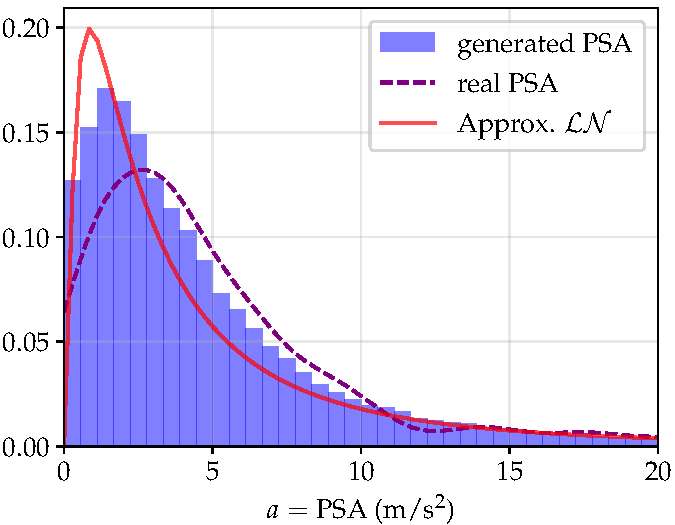
\includegraphics[width=5cm]{figures/intro-frags/PSA_density_withLN.pdf}\ 
    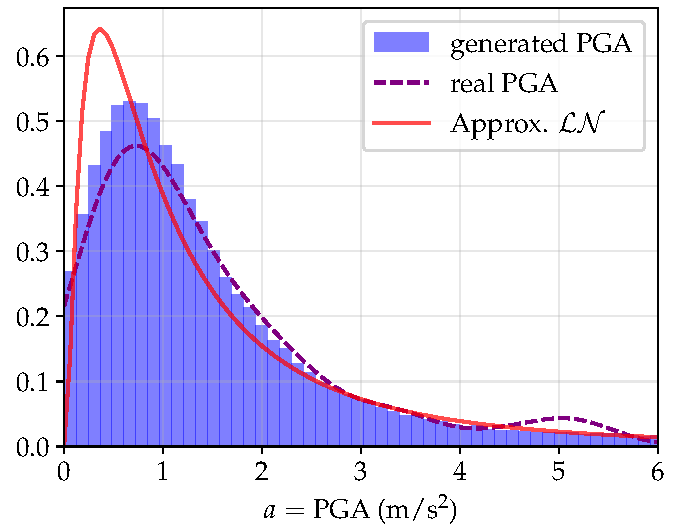
\includegraphics[width=5cm]{figures/intro-frags/PGA_density_withLN.pdf}
    \caption{Histograms of IMs derived from $10^5$ generated synthetic signals : the IM is the PSA (left) and the PGA (right). They are compared with the densities of IMs coming from real accelerograms estimated by Gaussian kernel estimation (dashed lines), {and with the densities of a lognormal distribution with same median and same log deviation (solid lines).}}
    \label{fig:intro-frags:IM-density}
\end{figure}



 %the conduction of 
%  the numerical experiments conducted 



%different IMs


% Regarding seismic ground motions, a common methodology



% SAinct et al

% definition of IMs


\subsubsection{Engineering demand parameter and failure}


As evoked in the preamble of this section, numerous data sources exist for identifying the fragility (and the failure) of mechanical structures and components.
In most cases a particular engineering demand parameter (EDP) of the system is focused on. The EDP is a scalar quantity that is observed (numerically or practically) during the seismic excitation, it can be the maximal displacement of a specific part of mechanical equipment for instance. More explicit examples will be given when specific case studies will be presented later on in this chapter. 
In those cases, the failure is defined when the EDP exceeds a threshold limit.

All in all, available datasets often take the form of tuples $((\cS_i,\cD_i))_{i=1}^k$, where $\cS_i$ is the $i$-th seismic signal submitted to the system and $\cD_i$ is the EDP that was observed during the experiment. %The reduced 
%
In the case studies that are treated in this manuscript a specific IM is chosen, and a reduced dataset of the form $((a_i,z_i))_{i=1}^k$ is studied, where $a_i$ is the IM of the $i$-th seismic signal, and $z_i=\indic_{\cD_i>\text{TH}}$, where $\text{TH}$ is the threshold that defines the failure of the system. In other words, $z_i=1$ if the system has failed when submitted to the  $i$-th seismic signal, and $z_i=0$ otherwise.
The dataset permits to statistically estimate the fragility curve of the system of interest. In this thesis, we restrict the study to cases where the observations can be considered independent. Naturally, that restriction excludes some case studies, such as experimental campaigns conducted on concrete structures for instance, since such system get damaged during the experiment, impacting their mechanical behavior. 
As mechanical systems that enter the scope of this thesis, we can cite
%\begin{itemize}
    % \item 
    structures and component  whose response under seismic excitation can be modeled numerically (via finite element analysis for instance), and
    % \item 
    sturdy mechanical equipments that do not get damaged during experimental campaigns such as pipes, electronic devices, stacked structures.
%\end{itemize}
In the last two examples evoked, the failure is not always characterized by observing an EDP, and can be multifactorial. While the studies that are done in this thesis are limited to cases where the system of interest's failure is characterized by an EDP, we emphasize that the methods that we develop and use go beyond these specific cases.



% However, structures and components whose response under seismic excitation can be modeled numerically via finite element methods are


% various mechanical equipment in the nuclear industry are sturdy enough 






\section{Modeling of the fragility curve}

Different models and methods have been suggested in the literature to estimate seismic fragility curves.
%Historically, the 
In the genesis of the SPRA, seismic fragility curves were estimated based on expert judgments, principally due to the scarcity of available data to conduct an accurate statistical estimation (see \cite{kennedy_probabilistic_1980}).
Of course, the accuracy of such an estimation is not guaranteed either, and its reliability depends on that of the experts.

Nowadays, estimates of seismic fragility curves are mostly derived using statistical techniques, leveraging (i) dataset that are sometimes less scarce and more precise, and also (ii) statistical techniques that are more efficient. 
The expert judgment still complement those in some works in the literature.


Parametric and non-parametric methods are both used in the literature to estimate seismic fragility curves.
In the former, the probabilistic relation between the failure and the IM is sought. When an EDP is available, authors seek to estimate first the probabilistic relation between the IM and the EDP, to deduce the resulting fragility curve.
In the latter, the fragility curve is assumed to belong to a parameterized set, reducing the problem to the estimation of these parameters.
While the first method is more general in the sense that it covers a wider range of possible estimates, it is also often less efficient than the second. Indeed, reducing the problem to a finite-parameter one allows providing satisfying estimates with fewer data. However, their reliability depends on the trustworthiness of the chosen parametric modeling.

In the following, we review briefly the
state-of-the art on the estimation of seismic fragility curves. We start by a review of non-parametric methods in section??. In that section we also describe a non-parametric estimation that is based on Monte-Carlo estimates, and that can serve as a reference when a large dataset is available.
In section?? we discuss the parametric modelings of the fragility curves, and we present the most common one: the probit-lognormal model.



% , in which we p



% Two main different approaches exist to model the fragility curve. Firstly, one approach consists in estimating 
% It is common to classify the modelings of fragility curves in two categories: the non-parametric ones and the pa








%\subsection{A state-of-the-art}





\subsection{Non-parametric modeling}


Most of non-parametric models for seismic fragility curves estimation leverage ---if possible--- the knowledge of an EDP that describes more precisely the response of the structure under seismic excitation than just the binary outcome ---failure or non-failure.
In this case it is possible to estimate the conditional distribution of the EDP to the IM (or IMs) via a surrogate modeling of the system $\text{EDP}=\cM(\text{IM})$.

Among common surrogates we can mention the Gaussian processes (GPs). As examples of their use for seismic fragility curves estimation, we can cite \cite{gidaris_kriging_2015}, in which GPs are used to estimate the EDP given multiple parameters characterizing the ground motion; and \cite{gauchy_uncertainty_2024}, in which the GPs-based estimation of the EDP is coupled with a sensitivity analysis of the fragility curve to the mechanical parameter of the studied system.

We also mention polynomial chaos expansion (PCE) as a surrogate numerously used for seismic fragility curves estimation. For instance, PCEs are combined in \cite{mai_surrogate_2016} with non-linear autoregressive with exogenous input models to estimate the temporal response of the mechanical system as a function of the seismic signal.
In \cite{zhu_surrogate_2023}, a stochastic PCE is conducted, consisting in the addition of a latent variable and an additive noise to the deterministic PCE expression.
%It is applied to the 

Outside surrogate modeling, what on would call machine-learning-based techniques are also implemented to estimate seismic fragility curves.
For examples, we quote linear regression or generalized linear regression \citep{lallemant_statistical_2015}, classification-based methods (see the review suggested in \cite{kiani_application_2019}) such as  logistic regression (as in \cite{bernier_fragility_2019}) or support vector machine (as in \cite{sainct_efficient_2020}). In the latter work, support vector machine is used to classify EDPs weather they led to failures or non-failures as a function of combinations of IMs.
We also mention artificial networks based methods, such as used in \cite{mitropoulou_developing_2011,wang_seismic_2018}.
 

% Of course, a

\subsubsection{A reference fragility curve constructed with a large dataset}

%All the methods cited above rely on assumptions on the probabilistic relation  between  the structure's response and the seismic excitation.
All the methods cited above provide estimation whose efficiency will depend on the size of the available dataset and the correctness of the assumptions they involve on the probability relation between the system's response and the IMs.
It is possible to minimize such assumptions considerably, trying to estimate directly the probabilities $\PP(\text{``failure''}|\text{IM}=a)$, for all value of $a$, via Monte-Carlo estimates for instance.
Such a methodology must give the best estimation of the fragility curve in terms of robustness, in the sense that it does not rely on any assumption. Of course, one does not have infinitely many data for all value of $a$ to provide an exact estimation of the whole curve, yet it is possible to approximate the curve locally in different sub-areas of the domain $\cA$ in which $a$ lives.
More explicitly consider a dataset $((a_i,z_i))_{i=1}^{N}$ of IMs and binary outcomes ($z_i=1$ if the $i$-th seismic signal led to a failure, and $0$ otherwise), and choose $N_c$ clusters of the $(a_i)_{i=1}^N$ that we denote $(K_j)_{j=1}^{N_c}$: $\bigsqcup_{j=1}^{N_c}K_j=\{a_i,$ $i=1,\dots,N\}$. Then it is possible to approximate the fragility curve evaluated at the centroids $(c_j)_{j=1}^{N_c}$ of the clusters:
    \begin{equation}
        P_f^{\text{MC}}(c_j) = \frac{1}{n_j}\sum_{i,\, a_i\in K_j}z_i,
    \end{equation}
where $n_j$ is the sample size of cluster $K_j$.
This non-parametric estimation is implemented by \citet{trevlopoulos_parametric_2019}, who suggest defining the clusters $(K_j)_{j=1}^{N_c}$ using K-means since the IM values in available datasets are generally not uniformly distributed.

When the number of available data is little and when they are poorly diverse in terms of values of the IM, this estimation method becomes limited for estimating seismic fragility curves. However, in the other case, we consider that it provides a robust result. %In this thesis, 
% In this thesis, when evaluating 
For this reason, while this thesis address the estimation of fragility curves when few data are available, we will evaluate our methods on case studies for which a large validation dataset exists.
The latter is used to derive what we call a reference fragility curve that is identified to $P^{\text{MC}}_f$, and which will be compared with the estimates provided by our methods.






%\subsection{Parametric modeling}

%probit lognormal



\subsection{Parametric modeling: probit-lognormal model}

\subsubsection{The probit-lognormal model}


Although based on stronger assumptions on the structure's response than non-parametric methods, parametric fragility curves were historically considered, especially in cases with small dataset limited to binary outcome (i.e. no EDP is available).
%Several model can 
In the SPRA and PBEE frameworks, the so-called probit-lognormal model was chosen, and it remains prevalent to this day (see e.g. \cite{shinozuka_statistical_2000,straub_improved_2008,zentner_numerical_2010,wang_influence_2020,mandal_seismic_2016,zhao_seismic_2020,ellingwood_earthquake_2001,kim_development_2004,mai_seismic_2017,trevlopoulos_parametric_2019,katayama_bayesian-estimation-based_2021,lee_efficient_2023}).
% This model is presented 
This model consists in introducing a parameter $\theta=(\alpha,\beta)$ and defining the fragility curve as follows
    \begin{equation}\label{eq:intro-frag:probit}
        P_f(a) = \PP(\text{``failure''}|\text{IM}=a) = \Phi\left( \frac{\log a-\log\alpha}{\beta} \right),
    \end{equation}
where $\Phi$ is the cumulative distribution function of a standard normal variable. An example of such curves is given in fig??.
We mention that, sometimes, the parametrization of the model is slightly different. As recalled by \cite{zentner_fragility_2017}, the distinguishing of epistemic and aleatoric uncertainty in $\beta$ is commonly suggested, leading to rewriting eq?? with $\beta=\sqrt{\beta^2_U+\beta^2_R}$. 
% The EPRI guide ?? suggested standard values 
The literature suggests that the uncertainty embedded in $\alpha$ is only epistemic.

\begin{figure}
    \caption{examples of probit lognormal fragility curves}
\end{figure}


Different strategies exist to estimate the two parameters, namely the median $\alpha$ and the log standard deviation $\beta$. Historically, maximum likelihood estimation (MLE) techniques are recommended.  %with confidence interval derivation via bootstrapping are recommended (see for instance ).
When the data are independent, the bootstrap technique can be used to obtain confidence intervals relating to the size of the sample considered (e.g. \cite{shinozuka_statistical_2000,zentner_numerical_2010,wang_influence_2020}). %, ZENTNER20101614, WangF2020}). 
% \cite{Shinozuka2000, ZENTNER20101614, WangF2020}. 
To describe this technique,
we define first the associated statistical model: the observations are modeled as realizations of the random variable $(A,Z)\in\cA\times\{0,1\}$. It is supposed that observations are independent conditionally to $\theta$ and that $(A,Z)$ are distributed conditionally to $\theta\in\Theta=(0,\infty)^2$ as:
    \begin{equation}
            A|\theta\sim A\sim H,\quad\text{and}\quad Z|A,\theta\sim\cB\left(\Phi\left(\beta^{-1}\log\frac{a}{\alpha}\right)\right)
    \end{equation}
where $H$ is the distribution of $A$ and $\cB(p)$ denotes a Bernoulli distribution of mean  $p$.
Thus, the likelihood $\ell_k$ given observations $(\mbf a^k,\mbf z^k)$ with $\mbf a^k=(a_i)_{i=1}^k$ and $\mbf z_k=(z_i)_{i=1}^{k}$ is expressed as
    \begin{equation}
        \ell_k(\mbf z^k,\mbf a^k|\theta) = \prod_{i=1}^k\ell(z_i,a_i|\theta) = \prod_{i=1}^k\Phi\left(\frac{\log a_i-\log\alpha}{\beta}\right)^{z_i}\left(1-\Phi\left(\frac{\log a_i-\log\alpha}{\beta}\right)^{1-z_i}\right)h(a_i),
    \end{equation}
where $h$ is the p.d.f. of $A$. Since the $(h(a_i))_i$ are constants of $\theta$ anad are not known in general, it is common to consider the following alternative form of the likelihood:
\begin{equation}
    \ell_k(\mbf z^k|\mbf a^k,\theta) = \prod_{i=1}^k\ell(z_i|a_i,\theta) = \prod_{i=1}^k\Phi\left(\frac{\log a_i-\log\alpha}{\beta}\right)^{z_i}\left(1-\Phi\left(\frac{\log a_i-\log\alpha}{\beta}\right)^{1-z_i}\right).
\end{equation}
The maximum likelihood estimator is $\theta^{\text{MLE}}(\mbf z^k,\mbf a^k)=\argmax_{\theta\in\Theta}\ell_k(\mbf z^k,\mbf a^k|\theta)$.
The bootstrap technique consists in deriving a stochastic estimator $\hat\theta_k^{\text{BMLE}}(\mbf z^k,\mbf a^k)$ whose distribution is defined from expressing it as: $\hat\theta^{\text{BMLE}}(\mbf z^k,\mbf a^k)=\theta^{\text{MLE}}((z_{U_i},a_{U_i})_{i=1}^k)$, where $U_1,\dots,U_k$ are i.i.d. random variables distributed w.r.t. a uniform distribution in $\{1,\dots,k\}$.



 
% we consider the statisct

% let us start by defining formally the statistical probit-lognormal model: 



\subsubsection{About the implementation of the Bayesian framework to estimate $\theta=(\alpha,\beta)$}

As a strategy that allows to estimate the parameters defining the fragility curve, 
the Bayesian framework has recently become increasingly popular in seismic fragility analysis (see e.g. \cite{gardoni_probabilistic_2002,wang_bayesian_2018,katayama_bayesian-estimation-based_2021,koutsourelakis_assessing_2010,damblin_approche_2014,tadinada_structural_2017,kwag_computationally_2018,jeon_parameterized_2019,tabandeh_physics-based_2020}). 
It is praised for its capacity to solve the irregularity issues encountered when estimating fragility curves with classical methods. For instance, the MLE-bootstrap method is known to lead to unrealistic estimates such as unit-step functions.
However, a challenge remains when %The difficulty that remains when 
implementing the Bayesian framework, and 
lies in the selection of the prior.
As a matter of fact, as announced since the \cref{chap:intro-english}, selecting a prior is a critical step in Bayesian analysis, %especially in a context where (i) the datasets of interest are light, and (ii) the methodology must be auditable.
and when exploring the literature, a wide range of different consideration can be found regarding its construction. % prior
%
%In earthquake engineering, Bayesian inference is often used to update existing log-normal fragility curves previously obtained through various approaches, assuming independent distributions for the prior values of $\alpha$ and $\beta$, such as log-normal distributions. 
%
For example, in \cite{tadinada_structural_2017} and \cite{kwag_computationally_2018}, the median prior values come from equivalent linearized mechanical models. In \cite{wang_bayesian_2018}, both aleatory and epistemic uncertainties are taken into account in the parametric model originally introduced in \cite{kennedy_probabilistic_1980}: an artificial neural network is trained and used to characterize (i) the aleatory uncertainty and (ii) the prior median value of $\alpha$, while the associated epistemic uncertainty is taken from the existing literature. The log-normal prior distribution of $\alpha$ is then updated with empirical data. 
In \cite{katayama_bayesian-estimation-based_2021}, the results of incremental dynamic analysis are used to obtain a prior value of $\alpha$, whereas the prior value of $\beta$ is determined through a parametric study. This results in satisfactory convergence, whatever its target value, before application to practical problems.
In \cite{straub_improved_2008}, the authors mainly focus on the implications for fragility analyses of statistical dependencies within the data. The prior is defined as the product of a normal distribution for $\ln(\alpha)$, and the improper distribution $1/\beta$ for $\beta$. The definition of the normal distribution is based on engineering assessments. This prior was preferred to $1/\alpha$ on the grounds that it led to unrealistically large posterior values of $\alpha$. A sensitivity analysis is further performed to examine the impact of the choice of the prior distribution on the final results.
Finally, we note that the Bayesian framework is also relevant for fitting numerical models (e.g., mathematical expressions based on engineering assessments or physics-based models) to experimental data in order to estimate fragility curves \citep{gardoni_probabilistic_2002,tabandeh_physics-based_2020} or meta-models such as logistic regressions \citep{koutsourelakis_assessing_2010,jeon_parameterized_2019}.







% In the SPRA framework, Bayesian inference is often used to update existing probit-lognormal fragility curves previously obtained through various approaches, assuming probit-lognormal distribution only for $\alpha$ \cite{WANG2018232}, 
% independent distributions for the prior values of $\alpha$ and $\beta$ such as uniform distributions \cite{KOUTSOURELAKIS2010}, the product of a normal distribution for $\ln(\alpha)$ and the improper distribution $1/\beta$ for $\beta$ \cite{Straub2008}, etc.


% in \cite{wang_bayesian_2018}, $\beta$ is replaced by in eq?? to 


%\cite{Shinozuka2000,Lallemant2015,Straub2008,ZENTNER20101614, WangF2020, MANDAL201611, WANGZ2018, WANG2018232, ZHAO2020103, ELLINGWOOD2001251, KIM2004, Mai2017, TREVLOPOULOS2019,Katayama2021,LEE2023}


\section{Example of case studies}

    \subsection{An elasto-plastic oscillator}

    The first case study that we present is 
    a single-degree-of-freedom elasto-plastic oscillator with kinematic hardening.
    %It represents a con
    This simple mechanical system illustrates the essential features which can be found in the nonlinear responses of some real-world structures under seismic excitation and has, for this reason, already been used in several studies~\cite{trevlopoulos_parametric_2019,sainct_efficient_2020,gauchy_importance_2021}.
    In addition, it provides reference results as a reasonable numerical cost.
    It is depicted in fig.??, 
    Its motion equation when submitted to an excitation $s$ is the following:
    \begin{equation}
        x''(t) +2\xi2\pi f_L x'(t)+f^{\text{nl}}(t) = -s(t),
    % \ddot{y}(t) + 2 \zeta \omega_{\text{L}}\dot{y}(t) + f(t) = -s(t) \ ,
    \end{equation}
    %with $s(t)$ a seismic signal, $\dot{y}(t)$ and $\ddot{y}(t)$ respectively the relative velocity and acceleration of the mass, 
    with $x''$ and $x'$ respectively the relative velocity and acceleration of the mass,  $\xi$ the damping ratio, $f_L$ the circular frequency, and $f^{\text{nl}}$ the nonlinear resisting force.

    \begin{figure}[h]
        \centering
        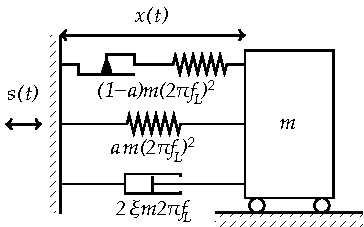
\includegraphics[width=6cm]{figures/intro-frags/KBEPO_rheo.pdf}
        \caption{Elasto-plastic oscillator of mass $m$ with kinematic hardening, with parameters $f_{\text{L}} = 5$ Hz and $\xi = 2\%$. The yield limit is $Y = 5.10^{-3}$~m, and the post-yield stiffness is $20\%$ of the elastic stiffness, i.e., $a = 0.2$.}   
    \end{figure}

    
    
    The relevant EDP is the absolute maximum value of the mass’ displacement, i.e., $\text{EDP}=\max_{t\in [0, T]}|x(t)|$, where $T$ is the duration of the seismic excitation.
    
    The failure criterion $\text{TH}$ is chosen to be the $90\%$-level quantile of the maximum displacement calculated with $10^5$ artificial signals, i.e., $C = 8.0 \; 10^{-3}$~m.
    Figure \ref{fig:ref-osci} compares the MC-based reference fragility curve $P_f^{\mathrm{MC}}$ (Eq.~(\ref{eq:refMC})) with its log-normal estimation $P_f^{\mathrm{MLE}}$, both estimated using the results of the $10^5$ simulations. In this case, the log-normal fragility curve is a good approximation of the reference curve.


    
    \subsection{A piping system from a pressurized water reactor}


s


    \subsection{Stacked structure for storage of packages: typical low data example}

s
    % \subsection{Appropriate modeling with how many data and what data}


\section{Which case study and which data for a Bayesian estimation of fragility curves?}

s


\section{Conclusion}


conclusion


